% Define document class
\documentclass[modern]{aastex631}
\usepackage{showyourwork}

\newcommand{\sbu}{Department of Physics and Astronomy, Stony Brook University, Stony Brook NY 11794, USA}
\newcommand{\cca}{Center for Computational Astrophysics, Flatiron Institute, New York NY 10010, USA}

\newcommand{\dd}{\mathrm{d}}
\newcommand{\order}[1]{\mathcal{O}\left( #1 \right)}

\newcommand{\bNS}{b_\mathrm{NS}}
\newcommand{\phiNS}{\phi_\mathrm{NS}}
\newcommand{\rNS}{r_\mathrm{NS}}
\newcommand{\vRot}{v_\mathrm{rot}}

\newcommand{\rSchw}{r_\mathrm{Schw}}

% Begin!
\begin{document}

% Title
\title{Lensing in the Schwarzschild Spacetime Applicable to Neutron Stars}

% Author list
\author[0000-0003-1540-8562]{Will M. Farr}
\email{wfarr@flatironinstitute.org}
\affiliation{\sbu}
\affiliation{\cca}

% Abstract with filler text
\begin{abstract}
    I describe the effects of gravitational lensing on the image of the surface
    of a spherical object whose surface is well outside the Schwarszchild
    horizon.
\end{abstract}

% Main body with filler text
\section{Introduction}
\label{sec:intro}

\section{Geodesics}
\label{sec:geodesics}

The Schwarzchild line element in standard coordinates and natural units is 
\begin{equation}
\dd s^2 = g_{\mu \nu} \dd x^\mu \dd x^\nu = - \left( 1 - \frac{2}{r} \right) \dd t^2 + \frac{1}{1 - \frac{2}{r}} \dd r^2 + r^2 \left( \dd \theta^2 + \sin^2 \theta \dd \phi^2\right);
\end{equation}
$t$ is the clock time of an observer at $r = \infty$, and $4\pi r^2$ is the area
of the constant-$r$, constant-$t$ hypersurfaces.  The Schwarzschild radius (the
coordinate of the event horizon) is $\rSchw = 2$ in these units.

The metric has two killing vectors, $\partial_t$ and $\partial_\phi$, since it
is independent of the corresponding coordinates.  Write
\begin{equation}
\partial_t = \xi^\mu \partial_\mu, \qquad \partial_\phi = \zeta^\mu \partial_\mu;
\end{equation}
then the only non-zero component of $\xi^\mu$ is $\xi^t = 1$, and the only
non-zero component of $\zeta^\mu$ is $\zeta^\phi = 1$.  If $p^\mu$ is the
momentum associated with a geodesic,
\begin{equation}
p^\mu = \frac{\dd \chi^\mu(\lambda)}{\dd \lambda},
\end{equation}
with $\lambda$ either proper time (for time-like geodesics) or an affine
parameter (null geodesics), and $\chi^\mu(\lambda)$ the coordinates of the
points on the geodesic, then N\"{o}ther's Theorem gives 
\begin{eqnarray}
\label{eq:conserved-e}
g_{\mu \nu} \xi^\mu p^\nu = - \left( 1 - \frac{2}{\chi^r} \right) p^t & = & \textnormal{const} \equiv - e,\\
\label{eq:conserved-l}
g_{\mu \nu} \zeta^\mu p^\nu = (\chi^r)^2 \sin^2 (\chi^\theta) p^\phi & = & \textnormal{const} \equiv l
\end{eqnarray}
along any geodesic.  ($e$ and $l$ are the energy and angular momentum---per unit
mass, if appropriate---of the particle traveling the geodesic measured by an
observer at infinity.)

For a null geodesic, we also have the normalization condition 
\begin{equation}
\label{normalization}
g_{\mu \nu} p^\mu p^\nu = 0.
\end{equation}
Exploiting the rotational symmetry of the $\theta$-$\phi$ subspace, we can,
without loss of generality, work in the equatorial plane, considering only
geodesics which have $\chi^\theta (\lambda) = \pi /2$.  In this case, Equation
\ref{normalization} becomes
\begin{equation}
    \label{eq:pr-normalization}
-\frac{e^2}{1 - \frac{2}{\chi^r}} + \frac{l^2}{(\chi^r)^2} + \frac{1}{1-\frac{2}{\chi^r}} \left( \frac{\dd \chi^r}{\dd \lambda} \right)^2 = 0.
\end{equation}
Rescaling the affine parameter, we obtain
\begin{equation}
\label{radial-path}
\frac{\dd \chi^r(s)}{\dd s} = \pm \sqrt{1 - \frac{b^2\left(1 - \frac{2}{\chi^r(s)} \right)}{(\chi^r(s))^2}},
\end{equation}
with $b \equiv l/e$ called the ``impact parameter''\footnote{$b$ is so named
because it gives the distance at infinity between the geodesic and the nearest
parallel line running radially from the center of the star.} of the trajectory.
This equation and Equations \ref{eq:conserved-e} and \ref{eq:conserved-l}
completely determine a trajectory given $l$ and $e$.  

\section{Intersection with the Surface}
\label{sec:surface}

For a given $b$, Equation \ref{radial-path} implies a point of closest approach
to the mass at 
\begin{equation}
\frac{\dd \chi^r(s_0)}{\dd s} = 0 = 1 - \frac{b^2 \left( 1 - \frac{2}{\chi^r\left(s_0\right)} \right)}{(\chi^r(s_0))^2}.
\end{equation}
This gives a cubic equation for $\chi^r(s_0)\equiv r_0$, whose solution is not
terribly illuminating.  Note that the ``point of closest approach'' may be
\emph{inside} the star if the impact parameter is small enough; in this case the
approach terminates at the stellar surface before achieving a close approach.

It is of interest to determine the impact parameter, $\bNS$, of the ``grazing
ray'' whose point of closest approach, $r_0$, is equal to the radius of the
neutron star, $\rNS$.  Noting $\rNS \gg 2$ for physical neutron stars, we have 
\begin{equation}
     \bNS^2 = \frac{\rNS^2}{1 - \frac{2}{\rNS}} = \rNS^2 \left( 1 + \frac{2}{\rNS} + \frac{4}{\rNS^2} + \ldots \right),
\end{equation}
or 
\begin{equation}
    \bNS = \rNS \left( 1 + \frac{1}{\rNS} + \frac{3}{2 \rNS^2} + \ldots \right).
\end{equation}
That the impact parameter of the grazing ray is \emph{larger} than the neutron
star radius is a result of gravitational lensing.  It is interesting that the
leading order addition to the impact parameter is one half the Schwarzschild
radius.

We wish to determine the longitude of the intersection of a ray with impact
parameter $b < \bNS$ and the surface; this is $\chi^\phi$, the $\phi$ coordinate
of the null geodesic, when the ray intersects the surface.  To do this, it will
be more convenient to parameterize the trajectory by $\chi^r$. Using the
trajectory derived in the last section (and remembering the scaling on the
affine parameter $s$), we have 
\begin{equation}
\frac{\dd \chi^\phi}{\dd \chi^r} = \frac{\dd \chi^\phi/\dd s}{\dd \chi^r/\dd s} = \frac{-b}{(\chi^r)^2 \sqrt{1 - \frac{b^2 \left(1 - \frac{2}{\chi^r} \right)}{(\chi^r)^2}}}.
\end{equation}
Thus, the longitude at ``impact'' is 
\begin{equation}
\chi^\phi\left( \rNS \right) = \int_{\rNS}^{\infty} \dd u \, \frac{b}{u^2 \sqrt{1 - \frac{b^2\left(1 - \frac{2}{u} \right)}{u^2 }}}.
\end{equation}
(The impact parameter of the grazing ray is $\bNS = \rNS\left( 1 + 1/\rNS +
\ldots \right)$, so the argument of the square root approaches zero for the
grazing ray at impact, but otherwise is guaranteed to be positive.)

It will be convenient to transform variables from $u$ to $w = u/\rNS$, whence 
\begin{equation}
    \label{eq:w-substitution}
    \chi^\phi\left( \rNS \right) = \int_{1}^{\infty} \dd w \, \frac{b}{\rNS w^2 \sqrt{1 - \frac{b^2\left(1 - \frac{2}{\rNS w} \right)}{\rNS^2 w^2}}}.
\end{equation}
It is also convenient to make the substitution 
\begin{equation}
    b = x \bNS = x \rNS \left( 1 + \frac{1}{\rNS} + \frac{3}{2 \rNS^2} + \ldots \right),
\end{equation}
whence $-1 < x < 1$ for rays that impact the neutron star surface. This produces 
\begin{equation}
    \chi^\phi\left( \rNS \right) = \int_1^\infty \dd w \, \frac{x \left( 1 + \frac{1}{\rNS} + \ldots \right)}{w^2 \sqrt{1 - \frac{x^2 \left( 1 + \frac{2}{\rNS} + \ldots \right)\left( 1 - \frac{2}{\rNS w} \right)}{w^2}}}.
\end{equation}

Expanding to leading order in $1/\rNS$, we obtain 
\begin{equation}
    \label{eq:chi-phi-impact}
    \chi^\phi\left( \rNS \right) = \arcsin x + \frac{2 \left( 1 - \sqrt{1-x^2} \right)}{x \rNS} + \ldots.
\end{equation}
We see that the grazing ray ($x = 1$) impacts the stellar surface at longitude 
\begin{equation}
    \phiNS = \frac{\pi}{2} + \frac{2}{\rNS} + \ldots = \frac{\pi}{2} + \frac{\rSchw}{\rNS} + \ldots
\end{equation}

It will be useful to have the momentum of the trajectory at the point of impact,
when $\chi^r = \rNS$, $\chi^\theta = \pi/2$, and $\chi^\phi$ given in Eq.\
\eqref{eq:chi-phi-impact}.  From Eq.\ \eqref{eq:conserved-e}, we see that 
\begin{equation}
    p^t = \frac{e}{1 - \frac{2}{\rNS}} \simeq e \left( 1 + \frac{2}{\rNS} + \ldots \right);
\end{equation}
from Eq.\ \eqref{eq:conserved-l}, and replacing the specific angular momentum
$l$ with the impact parameter $b = l/e$, we see that 
\begin{equation}
    p^\phi = \frac{b e}{\rNS^2} = \frac{x e}{\rNS} \left( 1 + \frac{1}{\rNS} + \ldots \right);
\end{equation}
and from Eq.\ \eqref{eq:pr-normalization}, we see that 
\begin{equation}
    p^r = e \sqrt{1 + \left( \frac{2 + 3 \rNS}{\rNS^3} - 1 \right) x^2} \simeq e \sqrt{1-x^2} \left( 1 + \frac{3 x^2}{2 \left( 1 - x^2 \right) \rNS^2} + \ldots \right).
\end{equation}

For a ray that does not approach the surface in the equatorial plane, but rather
strikes the surface at a colatitude $\theta_0$ (but still with impact parameter
$b = x \bNS$), the tangent vector $\phi$ component rotates into $\theta$ and
$\phi$ components, and the tangent is 
\begin{eqnarray}
    \label{eq:pt-final}
    p^t & \simeq & e \left( 1 + \frac{2}{\rNS} + \ldots \right) \\ 
    \label{eq:pr-final}
    p^r & \simeq & e \sqrt{1-x^2} \left( 1 + \ldots \right) \\
    \label{eq:ptheta-final}
    p^\theta & \simeq & \frac{x e \cos \theta_0}{\rNS} \left( 1 + \frac{1}{\rNS} + \ldots \right) \\
    \label{eq:pphi-final}
    p^\phi & \simeq & \frac{x e}{\rNS} \left( 1 + \frac{1}{\rNS} + \ldots \right),
\end{eqnarray}
where we have kept only terms $\order{1/\rNS}$ beyond leading order.

\section{Relativistic Effects on Energies}
\label{sec:relativistic}

For a neutron star that is observed to pulse with period $P$, observers at fixed
position on the surface follow coordinate trajectories in the body frame that
have 
\begin{eqnarray}
    \chi^\theta\left( \lambda \right) & = & \theta_0 \\
    \chi^r\left( \lambda \right) & = & \rNS \\
    \chi^\phi\left(\lambda \right) & = & \frac{2 \pi \chi^t\left(\lambda \right)}{P}
\end{eqnarray}
The last equation follows from the fact that $P$ is the proper time difference
between pulses arriving at infinity at fixed location on the celestial sphere;
and thus the \emph{coordinate} time difference between pulses is $\Delta t = P$.
(Beware!  This is not the \emph{proper} time between pulses as measured by
observers fixed to the neutron star surface; this latter quantity differs by a
gravitational redshift, a time dilation due to rotational motion, and a redshift
due to the radial acceleration of the rotational motion.)

The final coordinate trajectory for the fixed-position observer can be obtained
from the normalization condition:
\begin{equation}
    g_{\mu\nu} \frac{\dd \chi^\mu}{\dd \lambda} \frac{\dd \chi^\nu}{\dd \lambda} = -1,
\end{equation}
which fixes 
\begin{equation}
    \frac{\dd \chi^t}{\dd \lambda} = \frac{1}{\sqrt{1 - \frac{2}{\rNS} - \vRot^2 \sin^2 \theta_0}} = 1 + \frac{1}{2}  \vRot^2 \sin^2 \theta_0 + \frac{1 + \frac{3}{2} \vRot^2 \sin^2 \theta_0}{\rNS} + \ldots,
\end{equation}
where the last expansion is to first contributing order in $\vRot^2 = \left( 2
\pi \rNS / P \right)^2$ and $1/\rNS$.  In the expansion you can see the effects
of special relativistic time dilation, the gravitational redshift, and the
radial acceleration (the latter being proportional to $\vRot^2 / \rNS$).  Since
this expression is constant, the coordinate time of the observer increases
linearly (but not with coefficient equal to one) with proper time:
\begin{equation}
    \Delta \chi^t = \Delta \lambda \frac{\dd \chi^t}{\dd \lambda}.
\end{equation}

To convert this world-line tangent vector to the \emph{observer} coordinate
system, let the inclination of the neutron star spin be $\iota$ and the
obliquity (measered ccw from ``vertical'' in the observer frame) be $\omega$.
Then the neutron star spin three-vector has cartesian components in the observer
frame of 
\begin{equation}
    \vec{s} = \left( \cos \iota, -\sin \iota \sin \omega, \sin \iota \cos \omega \right).
\end{equation}
See the Figure \ref{fig:obs_cart}.
%%%
\begin{figure}
    \centering
        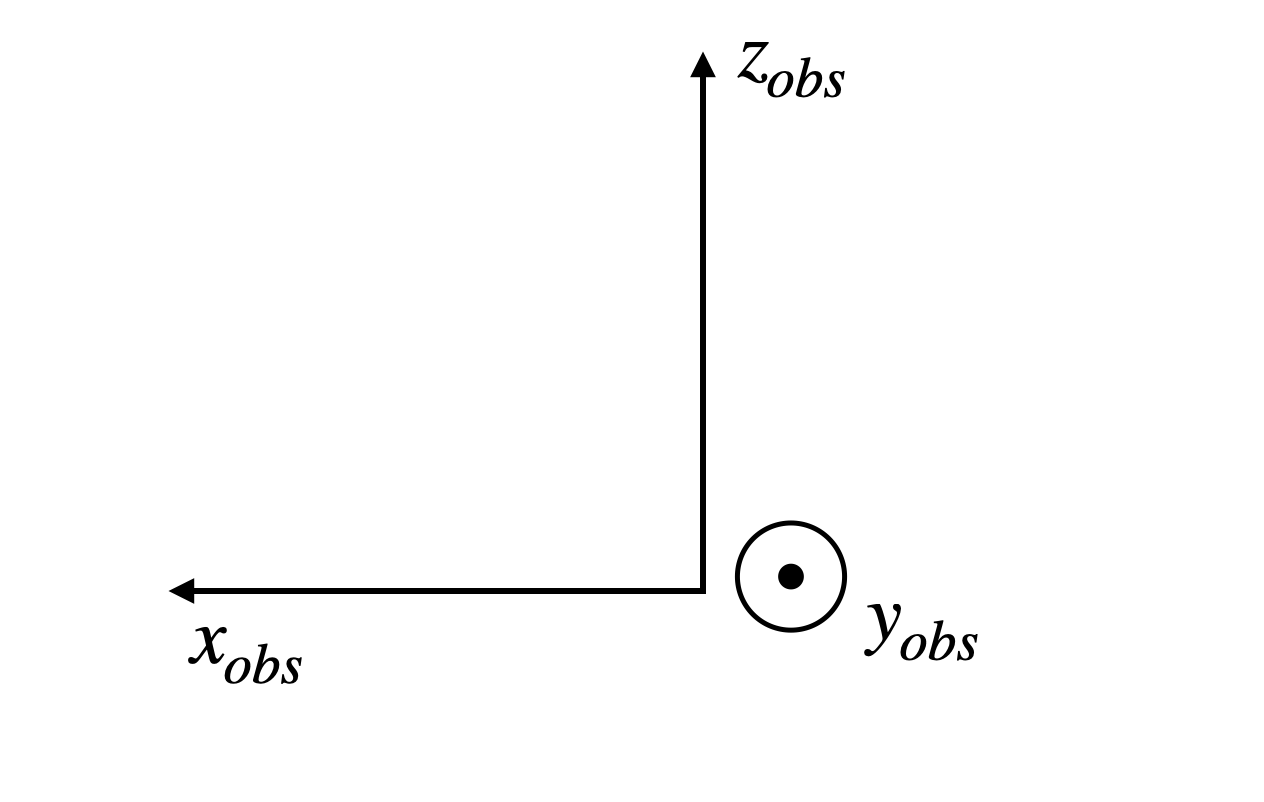
\includegraphics[width=0.9\columnwidth]{obs_cart_coord.png}
        \caption{The coordinates in the observer frame.}
        \label{fig:obs_cart}
    \end{figure}
%%%
If the incoming ray strikes the surface at a point with colatitude $\theta_0$
and longitude $\phi_0$, then the vector pointing to the impact point has
cartesian components in the observer frame of 
\begin{equation}
    \vec{r}_0 = \left( \cos \phi_0 \sin \theta_0, \sin\phi_0 \sin \theta_0, \cos \theta_0 \right).
\end{equation}
The instantaneous world-line tangent of the observer fixed to the NS surface at
the point of impact is given in cartesian coordinates by -- IT IS THE AZIMUTHAL VELOCITY? 
\begin{equation}
    \label{eq:tangent_vel}
    \vec{t}_0 = \frac{2 \pi r_{NS}}{P} \frac{\partial \chi^t}{\partial \lambda} \vec{s} \times \vec{r}_0. 
\end{equation}

The cross product is 
\begin{align*}
    % \begin{equation}
        \vec{s} \times \vec{r}_0 = \left(
        -\sin \iota \sin \omega \cos \theta_0 - \sin \iota \cos \omega \sin\phi_0 \sin \theta_0, \right. \\
        \left. \cos \iota \cos \theta_0 - \sin \iota \cos \omega \cos \phi_0 \sin \theta_0, \right. \\
        \left. \cos \iota \sin\phi_0 \sin \theta_0 + \sin \iota \sin \omega \cos \phi_0 \sin \theta_0 \right)
    % \end{equation}  
\end{align*}
    

Plugging in the cross product into the equation \ref{eq:tangent_vel} and solving for $r-, \theta-, \phi-$ components of the vector, then, in the observer spherical coordinate system the components of the tangent vector
are given by 
\begin{eqnarray}
    \frac{\mathrm{d}\chi^t}{\mathrm{d} \lambda} & \simeq & 1 + \frac{1}{2}  \vRot^2 \sin^2 \theta_0 + \frac{1 + \frac{3}{2} \vRot^2 \sin^2 \theta_0}{\rNS} \\
    \frac{\mathrm{d} \chi^r}{\mathrm{d} \lambda} & = & 0 \\
    \frac{\mathrm{d} \chi^\theta}{\mathrm{d} \lambda} & = & \frac{\mathrm{d} \chi^t}{\mathrm{d}\lambda} \frac{2\pi}{P} \left( - \cos\iota \sin \phi_0 - \cos\phi_0 \sin \iota \sin \omega \right) \\
    \frac{\mathrm{d} \chi^\phi}{\mathrm{d} \lambda} & = & \frac{\mathrm{d} \chi^t}{\mathrm{d}\lambda} \frac{2\pi}{P} \left( -\cos\iota \cos \phi_0 \cot \theta_0  + \sin \iota \left( \cos \omega + \cot \theta_0 \sin \phi_0 \sin \omega \right) \right)
\end{eqnarray}

[I have only worked out the geometry up to here.]

For a photon striking the surface of the neutron star with momentum $p^\mu\left(
e, l \right)$, the energy measured by the observer fixed to the surface is 
\begin{equation}
    -e_\mathrm{surf} = g_{\mu\nu} \frac{\dd \chi^\mu}{\dd \lambda} p^\nu.
\end{equation}
If we reverse the spatial components of the momentum, then for a photon
\emph{emitted} from the surface with energy $e_\mathrm{surf}$ in the frame fixed
to the stellar surface (e.g.\ thermally from particles on the surface), the
above equation relates the emitted energy to the energy as measured by observers
at infinity ($e$).

Plugging in Eqs.\ \eqref{eq:pt-final}, \eqref{eq:pr-final},
\eqref{eq:ptheta-final}, and \eqref{eq:pphi-final}, remembering to reverse the
spatial components of the momentum, we obtain the relation between the energy
observed at infinite distance ($e$) and the emitted energy at the surface
($e_\mathrm{surf}$) for a ray with impact factor $b = x \bNS$ hitting the
surface of the neutron star at colatitude $\theta_0$:
\begin{multline}
    \label{eq:energy-relation}
    \frac{e}{e_\mathrm{surf}} = 1 - y \vRot \sin \theta_0 + \left( y^2 - \frac{1}{2} \right) \vRot^2 \sin^2 \theta_0 \\ 
    - \frac{1}{\rNS} \left( 1 - \left( y^2 - \frac{1}{2} \right) \vRot^2 \sin^2 \theta_0 \right) + \ldots, 
\end{multline}
where $y = x \sin \theta_0$ is the ``equatorial'' component of the
(dimensionless) impact factor.  (Recall $x, y < 0$ for points west of the
meridian and $x, y > 0$ for points to the east; $\sin \theta_0 > 0$ always
because $0 < \theta_0 < \pi$.)

The velocity-independent term in Eq.\ \eqref{eq:energy-relation} gives the
gravitational redshift; the term linear in velocity gives the doppler shift from
the rotational motion (blueshift---increased energy---west of the meridian,
redshift---decreased energy---for points to the east); and the term quadratic in
the velocity comes from relativistic beaming.

\section{Calculating the time delay}
%
\begin{linenomath}\begin{align}
    \label{eq:geodesic}
    ds^2 = g_{\mu\nu}dx^\mu dx^\nu = -(1-\frac{2}{r})dt^2 + \frac{1}{1-\frac{2}{r}}dr^2 + r^2(d\theta^2+\sin^2 \theta d\phi^2)
\end{align}\end{linenomath}
%
\begin{linenomath}\begin{align}
    \label{eq:momentum}
    p^\mu = \frac{d\chi^\mu(\lambda)}{d\lambda}
\end{align}\end{linenomath}
%

In order to calculate the time delay, we need to calculate $\frac{d\chi^t(\lambda)}{d\lambda}$ and $\frac{d\chi^r(\lambda)}{d\lambda}$. Then, the time delay
can be calculated as 
%
\begin{linenomath}\begin{align}
    \label{eq:timedelay}
    \Delta t = \int_{r_{NS}}^{\infty} dr \left(\frac{d\chi^t}{d\chi^r} - \frac{d\chi^t}{d\chi^r}\vert_{b=0} \right)
\end{align}\end{linenomath}
%

Let's calculate $\frac{d\chi^t(\lambda)}{d\lambda}$ and $\frac{d\chi^r(\lambda)}{d\lambda}$ assuming $\theta=\pi/2$ and therefore $p^\theta = 0$. The we have
in null geodesic:
%
\begin{linenomath}\begin{align}
    \label{eq:nullgeo}
    -(1-\frac{2}{r})(p^t)^2 + \frac{1}{1-\frac{2}{r}}(p^r)^2 + r^2\sin^2 \theta (p^\phi)^2 = 0
\end{align}\end{linenomath}
%
Solving eq. \ref{eq:nullgeo} leads to $p^t = \frac{d\chi^t(\lambda)}{d\lambda} = \frac{e}{1-\frac{2}{r}}$ and 
%
\begin{linenomath}\begin{align}
    \label{eq:pr-squared}
    \left(\frac{d\chi^r(\lambda)}{d\lambda}\right)^2 = \left(\frac{e^2}{1-\frac{2}{r}} - \frac{l^2}{r^2}\right) \left(1-\frac{2}{r}\right)
\end{align}\end{linenomath}
%
which, in terms of $b$ becomes
%
\begin{linenomath}\begin{align}
    \label{eq:pr-b}
    \frac{d\chi^r(\lambda)}{d\lambda} = e\sqrt{\left(\frac{1}{1-\frac{2}{r}} - \frac{b^2}{r^2}\right) \left(1-\frac{2}{r}\right)}
\end{align}\end{linenomath}
%
Therefore, the integral \ref{eq:timedelay} becomes:
%
\begin{linenomath}\begin{align}
    \label{eq:timedelayfull}
    \Delta t = \int_{r_{NS}}^{\infty} dr \left[\left(\frac{1}{1-\frac{2}{r}}\right) - \frac{1}{\sqrt{\left(1-\frac{2}{r}\right)^2 - \frac{b^2}{r^2}\left(1-\frac{2}{r}\right)^3}}\right]
\end{align}\end{linenomath}
%
Following the substitution in Eq. \ref{eq:w-substitution}, we then get
%
\begin{linenomath}\begin{align}
    \label{eq:tdelay-with-w}
    \Delta t = r_{NS} \int_{1}^{\infty} \mathrm{d} w \, \left[\left(\frac{1}{1-\frac{2}{wr_{NS}}}\right) - \frac{1}{\sqrt{\left(1-\frac{2}{wr_{NS}}\right)^2 - \frac{b^2}{(wr_{NS})^2}\left(1-\frac{2}{wr_{NS}}\right)^3}}\right]
\end{align}\end{linenomath}
%
It is also convenient to make the substitution 
\begin{equation}
    b = x \bNS = x \rNS \left( 1 + \frac{1}{\rNS} + \frac{3}{2 \rNS^2} + \ldots \right),
\end{equation}
which produces 
%
\begin{linenomath}\begin{align}
    \label{eq:tdelay-with-x}
    \Delta t = r_{NS} \int_{1}^{\infty} \mathrm{d}w \, \left[\left(\frac{1}{1-\frac{2}{wr_{NS}}}\right) - \frac{1}{\sqrt{\left(1-\frac{2}{wr_{NS}}\right)^2 - \frac{x^2 \rNS^2 \left( 1 + \frac{1}{\rNS} + \frac{3}{2 \rNS^2} + \ldots \right)^2}{(wr_{NS})^2}\left(1-\frac{2}{wr_{NS}}\right)^3}}\right]
\end{align}\end{linenomath}
%
Substituting $1/r_{NS} = y$, and expanding around $y=0$, the integral gives
%
\begin{multline}
    \label{eq:tdelay-solved}
    \Delta t = r_{NS} \left( -1 + \sqrt{1 - x^2} \right) \\ \times \left( 1 + \frac{1}{r_{NS}} \left( 1  + \frac{2}{-1 + \sqrt{1 - x^2}} \log\left( \frac{x^2}{2 - 2 \sqrt{1 - x^2}} \right) \right) + \mathcal{O}\left( \frac{1}{r_{NS}^2} \right) \right)
\end{multline}
where $-1<x<1$.

\section{Creating matrix E for the energy factor}
To express the expression in \ref{eq:energy-relation} in matrix form using the spherical harmonic basis, we need to define matrices 
that correspond to the spherical harmonic functions and their associated coefficients. 

Let's denote the spherical harmonic basis as $Y_{lm}(\theta, \phi)$. The spherical harmonic basis is expressed as:
\begin{equation}
    \label{eq:spherical-harmonics}
    Y_{lm}(\theta, \phi) = P_{lm}(\theta, \phi) \cdot e^{i \cdot m \cdot \phi}
\end{equation}

where $P_{lm}(\theta, \phi)$ are the associated Legendre polynomials.

To express the given expression in matrix form using the spherical harmonic basis, we need to expand the function \( F(y, v_{\text{rot}}, \theta_0, r_s) \) 
into a series of spherical harmonic functions and their coefficients. The general form of the spherical harmonic expansion is:

\begin{equation}
    F(y, v_{rot}, \theta_0, r_s) = \sum_{l=0}^{\infty} \sum_{m=-l}^{l} C_{lm} Y_{lm}(\theta, \phi) 
\end{equation}

% Now, let's break down the given function step by step:

% \begin{multline}
%     F(y, v_{rot}, \theta_0, r_s) &= 1 - yv_{\text{rot}}\sin{\theta_0} + (y^2 - \frac{1}{2})v_{\text{rot}}^2\sin^2{\theta_0} - \frac{1}{r_s}\left(1-(y^2 - \frac{1}{2})v_{\text{rot}}^2\sin^2{\theta_0}\right) \\
%     = 1 - yv_{\text{rot}}\sin{\theta_0} + (y^2 - \frac{1}{2})v_{\text{rot}}^2\sin^2{\theta_0} - \\ \frac{1}{r_s} + \frac{(y^2 - \frac{1}{2})v_{\text{rot}}^2\sin^2{\theta_0}}{r_s} Y_{lm}(\theta, \phi) = P_{lm}(\theta, \phi) \cdot e^{i \cdot m \cdot \phi}
% \end{multline}

Now, the spherical harmonic expansion involves integrating \( F \) against each spherical harmonic function \( Y_{lm} \). 
The coefficients \( C_{lm} \) can be found using the following formula:

\begin{linenomath}\begin{align}
    C_{lm} = \int F(y, v_{rot}, \theta_0, r_s) \cdot Y_{lm}^*(\theta, \phi) \, d\Omega 
\end{align}\end{linenomath}

Here's how the matrix elements are formed:

\begin{linenomath}\begin{align}
C_{lm} = \int F(y, v_{\text{rot}}, \theta_0, r_s) \cdot Y_{lm}^*(\theta, \phi) \, d\Omega 
\end{align}\end{linenomath}

For \( C_{00} \) (the \( l = 0, m = 0 \) component):

\begin{linenomath}\begin{align}
    C_{00} = \int F(y, v_{\text{rot}}, \theta_0, r_s) \cdot Y_{00}^*(\theta, \phi) \, d\Omega = \int F(y, v_{\text{rot}}, \theta_0, r_s) \, d\Omega 
\end{align}\end{linenomath}


In the spherical harmonic basis, we can express the coefficients of the basis functions in matrix form:

\begin{multline}
    \mathbf{C} = \begin{bmatrix}
    1 & -v_{\text{rot}}\sin{\theta_0} & v_{\text{rot}}^2\sin^2{\theta_0} - \frac{1}{r_s} & 0 & \ldots \\
    0 & y\sqrt{2}v_{\text{rot}}\sin{\theta_0} & 0 & \ldots & \ldots \\
    0 & 0 & (y^2 - \frac{1}{2})\sqrt{6}v_{\text{rot}}^2\sin^2{\theta_0} & \ldots & \ldots \\
    0 & 0 & 0 & \ldots & \ldots \\
    \ldots & \ldots & \ldots & \ldots & \ldots \\
    \end{bmatrix}
\end{multline}

Here, the rows of the matrix correspond to different values of "l" and the columns correspond to different values of "m". 
The diagonal elements of the matrix correspond to the coefficients of the spherical harmonic basis functions with the same "l" and "m" values, 
while off-diagonal elements are zero.

Spherical harmonics for \(m = -1\), \(m = 0\), and \(m = 1\):
$$Y_{l,-1}(\theta, \phi) = \sqrt{\frac{3}{8\pi}}e^{-i\phi}\sin\theta$$
$$Y_{l,0}(\theta, \phi) = \sqrt{\frac{3}{4\pi}}\cos\theta$$
$$Y_{l,1}(\theta, \phi) = -\sqrt{\frac{3}{8\pi}}e^{i\phi}\sin\theta$$

Matrix elements for \(m = -1\):
$$M_{-1} = -\sqrt{\frac{3}{8\pi}}v_{\text{rot}}e^{-i\phi_0}\sin\theta_0$$

Matrix elements for \(m = 0\):
$$M_{0} = -\frac{\sqrt{6}}{2}v_{\text{rot}}^2e^{-2i\phi_0}\sin^2\theta_0$$

Matrix elements for \(m = 1\):
$$M_{1} = -\sqrt{\frac{3}{8\pi}}v_{\text{rot}}^2e^{-2i\phi_0}\sin^2\theta_0$$

\begin{multline}
    \begin{bmatrix}
        1 & -yv_{\text{rot}}\sin\theta_0 & (y^2 - \frac{1}{2})v_{\text{rot}}^2\sin^2\theta_0 - \frac{1}{r_s}(1 - (y^2 - \frac{1}{2})v_{\text{rot}}^2\sin^2\theta_0) \\
        0 & -\sqrt{\frac{3}{8\pi}}v_{\text{rot}}e^{-i\phi_0}\sin\theta_0 & -\frac{\sqrt{6}}{2}v_{\text{rot}}^2e^{-2i\phi_0}\sin^2\theta_0 \\
        0 & 0 & -\sqrt{\frac{15}{8\pi}}v_{\text{rot}}^2e^{-2i\phi_0}\sin^2\theta_0
    \end{bmatrix}
\end{multline}


\bibliography{bib}

\end{document}
